%---------------------- Problema 2 ------------------------------
\newpage
\section*{Problema 2}

\begin{enunciado}{Problema 2 (4 puntos)}
    Se pretende dise\~nar una estructura met\'alica para un paradero de buses.
    Como condici\'on de dise\~no, la estructura debe estar compuesta por vigas
    de acero ($E = 206$ GPa, $G = 80$ GPa y $S_y = 300$ MPa) y la misma debe
    cubrir como m\'inimo una superficie de 4 m x 2 m y una altura de 2 m. Las
    vigas a utilizar en la estructura son tubos de di\'ametro externo 30 mm y
    espesor 3 mm. No hay limitaci\'on en el dise\~no en cuanto al n\'umero de
    vigas que componen la estructura. En el c\'alculo por MEF, considerar que
    la \'unica fuerza actuante es el peso propio de las vigas el cual se
    supondr\'a distribuido a lo largo de las mismas ($\rho = 7800$ kg/m$^3$ y
    $g = 9.8$ m/s$^2$). Como restricci\'on de dise\~no, se pide que la tensi\'on
    en ninguna de las barras supere el l\'imite el\'astico y, adem\'as, que la
    deflexi\'on m\'axima sea menor a un valor dado ($\delta_{max} = 10$ mm).
\end{enunciado}

\vspace{0.5cm}

%---------------------- Desarrollo -------------------------------

\begin{desarrollo}{Propiedades de la sección y carga}
El tubo tiene radio exterior $r_e=15$ mm y radio interior $r_i=12$ mm:
$$A=\pi\,(r_e^2-r_i^2)=254.5\ \text{mm}^2,\qquad
I=\frac{\pi}{4}\,(r_e^4-r_i^4)=23\,475\ \text{mm}^4,\qquad
J=2I=46\,950\ \text{mm}^4$$
Como la sección es circular, $I_x=I_y=I$ y la orientación de los ejes locales
de cada barra no afecta la rigidez. El peso propio es una carga uniforme
vertical sobre todas las barras:
$$q=\rho\,g\,A=7800\cdot 9.8\cdot 254.5\times10^{-6}=19.45\ \text{N/m}$$
\end{desarrollo}

\begin{desarrollo}{Propuesta de diseño}
La estructura cubre exactamente el mínimo pedido: un techo de
$2\times4$ m (ejes $x$ e $y$) a $h=2$ m de altura. Se compone de:
\begin{itemize}[itemsep=2pt]
    \item \textbf{Marco de techo} de 6 barras: los dos largueros de 4 m
    ($y$) y los lados cortos de 2 m ($x$), cada uno partido en su punto
    medio (nodos 8 y 9).
    \item \textbf{Columnas delanteras} verticales en $x=2$ m (nodos 1--5 y
    2--6).
    \item \textbf{Columnas traseras inclinadas}: nacen en las esquinas
    traseras del suelo (nodos 0 y 3) y llegan al punto medio de los lados
    cortos del techo (nodos 8 y 9). Así la parte trasera queda libre en el
    suelo y la columna trabaja inclinada, como un puntal.
    \item \textbf{Atiesadores laterales} (ver iteración de diseño): barras
    cortas de 0.92 m que unen cada columna inclinada a $z=1.4$ m (nodos 10
    y 11) con la esquina trasera del techo (nodos 4 y 7). Están en los
    planos laterales $y=0$ e $y=4$ m, por lo que no tapan la vista frontal
    ni la trasera del paradero.
\end{itemize}
Las cuatro bases (nodos 0 a 3) se consideran empotradas (6 GDL
restringidos cada una), como una placa base apernada a un poyo de hormigón.

\begin{center}
\renewcommand{\arraystretch}{1.15}
\small
\begin{tabular}{cc@{\hspace{1.5cm}}cc}
\hline
Nodo & $(x,y,z)$ [m] & Nodo & $(x,y,z)$ [m]\\
\hline
0 & $(0,0,0)$ & 6  & $(2,4,2)$\\
1 & $(2,0,0)$ & 7  & $(0,4,2)$\\
2 & $(2,4,0)$ & 8  & $(1,0,2)$\\
3 & $(0,4,0)$ & 9  & $(1,4,2)$\\
4 & $(0,0,2)$ & 10 & $(0.7,0,1.4)$\\
5 & $(2,0,2)$ & 11 & $(0.7,4,1.4)$\\
\hline
\end{tabular}
\end{center}

\begin{center}
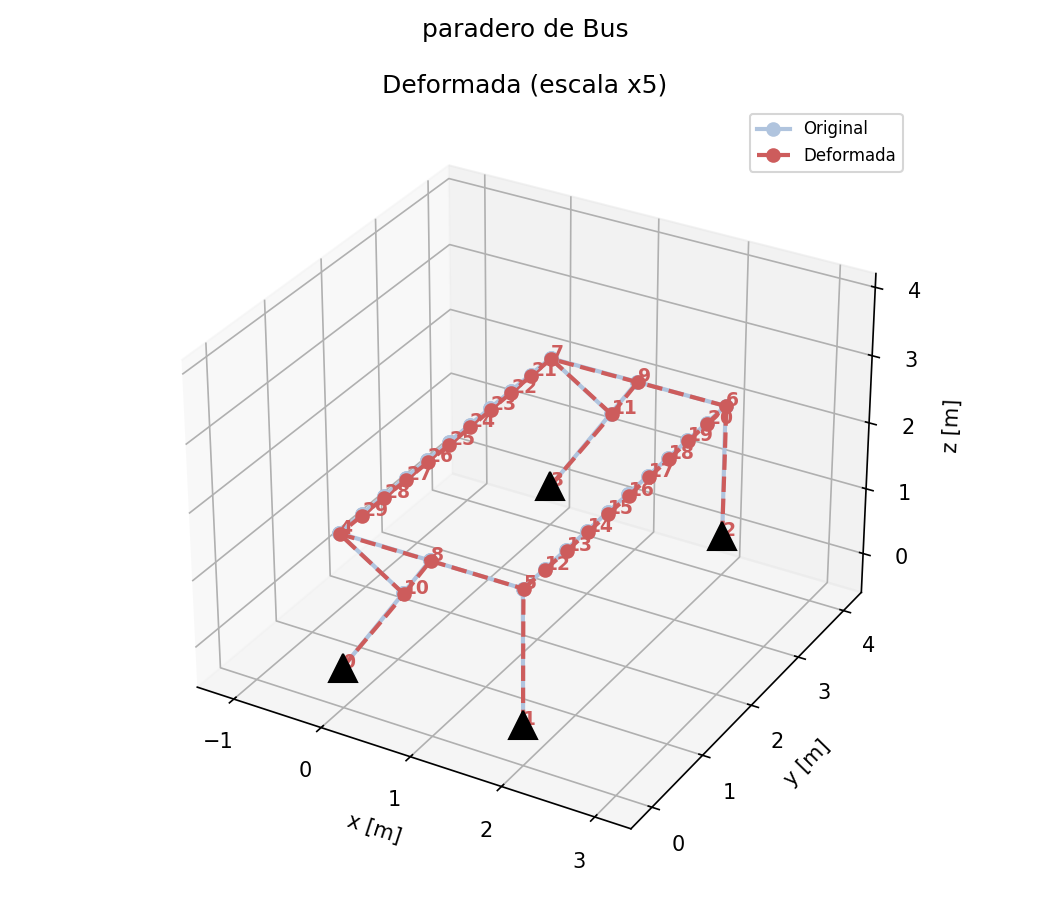
\includegraphics[width=0.75\linewidth]{T2/figuras_P2/deformada.png}
\captionof{figure}{Diseño final del paradero con la numeración de nodos y la
deformada amplificada 5 veces. Los nodos 12--29 son los nodos interiores de
los largueros de 4 m.}
\label{fig:t2-p2-deformada}
\end{center}

La longitud total de tubo es de 22.32 m, con un peso de 434.1 N
($\approx 44.3$ kg).
\end{desarrollo}

\begin{desarrollo}{Modelo de elementos finitos}
Se usan elementos de viga 3D de dos nodos (6 GDL por nodo:
$u_x,u_y,u_z,\theta_x,\theta_y,\theta_z$), con las mismas funciones del
Problema 1 (archivo \texttt{Problema\_2.py}):
\begin{itemize}[itemsep=2pt]
    \item \textbf{Rigidez:} matriz de viga de $12\times12$ en ejes locales
    (axial, dos flexiones de Hermite y torsión), llevada a ejes globales con
    $\mathbf{K}_e=\mathbf{T}^T\mathbf{k}_e\mathbf{T}$ y ensamblada en
    $\mathbf{K}$.
    \item \textbf{Peso propio como cargas nodales:} el peso de cada elemento
    se reemplaza por fuerzas y momentos concentrados en sus dos nodos, que se
    aplican igual que cargas puntuales (archivo \texttt{cargas\_nodales.py}).
    Para un elemento de nodos $i$--$j$, con $\mathbf{d}=\mathbf{x}_j-\mathbf{x}_i$,
    $l=|\mathbf{d}|$ y $\mathbf{q}=(0,0,-q)$:
    $$\mathbf{F}_i=\mathbf{F}_j=\frac{\mathbf{q}\,l}{2},\qquad
    \mathbf{M}_i=\frac{l}{12}\,(\mathbf{d}\times\mathbf{q}),\qquad
    \mathbf{M}_j=-\mathbf{M}_i$$
    Cada nodo recibe la mitad del peso del elemento, y los momentos tienen
    módulo $q_\perp l^2/12$ ($q_\perp$ es la componente del peso perpendicular
    a la barra) alrededor del eje horizontal perpendicular a ella. En una
    columna vertical $\mathbf{d}\times\mathbf{q}=\mathbf{0}$, así que solo hay
    fuerza. Las cargas de todos los elementos se suman en cada nodo.
    \item \textbf{Malla:} los dos largueros de 4 m se dividen en 10
    elementos cada uno. Así se obtiene la flecha en su centro, que es donde
    se espera la deflexión máxima. Las demás barras se modelan con un
    elemento. Como toda la carga queda en los nodos, los esfuerzos se
    calculan con $\mathbf{f}=\mathbf{k}_e\mathbf{u}_e$: dentro de cada
    elemento el corte y la axial son constantes y el momento es lineal.
\end{itemize}

Cargas nodales resultantes en los nodos principales (los nodos 0--3 son
apoyos y su carga pasa directo a la reacción):
\begin{center}
\renewcommand{\arraystretch}{1.15}
\small
\begin{tabular}{cccc}
\hline
Nodo & $F_z$ [N] & $M_x$ [N$\cdot$m] & $M_y$ [N$\cdot$m]\\
\hline
4, 7   & $-22.58$ & $\mp0.259$ & 2.667\\
5, 6   & $-33.07$ & $\mp0.259$ & $-1.621$\\
8, 9   & $-25.98$ & 0 & $-0.326$\\
10, 11 & $-30.71$ & 0 & $-2.496$\\
\hline
\end{tabular}
\end{center}
En los 18 nodos interiores de los largueros llega $F_z=-q\cdot0.4=-7.78$ N y
el momento es cero, porque los momentos de los dos elementos vecinos (de igual
largo) son iguales y opuestos. La suma de todas las fuerzas nodales es
$-434.08$ N, que es el peso total de la estructura.

El modelo queda con 30 nodos y 32 elementos: 180 GDL, de los cuales 24
están restringidos y 156 son libres. La matriz reducida tiene rango 156,
así que la estructura es estable.

\textbf{Verificación del equilibrio.} Las reacciones verticales suman
$\sum R_z=434.08$ N, que es el peso total de las barras, y
$\sum R_x=\sum R_y=0$:
\begin{center}
\renewcommand{\arraystretch}{1.15}
\small
\begin{tabular}{ccccccc}
\hline
Nodo & $R_x$ [N] & $R_y$ [N] & $R_z$ [N] & $M_x$ [N$\cdot$m] & $M_y$ [N$\cdot$m] & $M_z$ [N$\cdot$m]\\
\hline
0 & 9.50  & 14.85  & 126.84 & $-8.70$ & $-32.55$ & 4.61\\
1 & $-9.50$ & 14.55  & 90.20  & $-9.70$ & $-9.59$  & 0.27\\
2 & $-9.50$ & $-14.55$ & 90.20  & 9.70  & $-9.59$  & $-0.27$\\
3 & 9.50  & $-14.85$ & 126.84 & 8.70  & $-32.55$ & $-4.61$\\
\hline
Suma & 0 & 0 & 434.08 & & & \\
\hline
\end{tabular}
\end{center}
Las reacciones son simétricas respecto del plano $y=2$ m, igual que la
estructura. Las bases traseras toman más carga (127 N contra 90 N) porque
reciben el lado trasero del techo más las columnas inclinadas y los
atiesadores.
\end{desarrollo}

\begin{desarrollo}{Iteración de diseño: atiesadores}
La primera versión del diseño no tenía atiesadores. En ella las esquinas
traseras del techo (nodos 4 y 7) solo se apoyaban en los tramos de 1 m que
van a la punta de las columnas inclinadas. El larguero trasero de 4 m
quedaba colgando de dos voladizos y su centro bajaba \textbf{15.08 mm}, lo
que \emph{no cumple} $\delta_{max}=10$ mm. Las tensiones sí cumplían
($\sigma_{VM}=34.5$ MPa).

Para corregirlo sin cambiar la idea del diseño ni tapar la vista, se agregó
un atiesador en cada cara lateral. Este apoya la esquina trasera del techo
directamente sobre la columna inclinada. Se evaluó la altura $z_{at}$ a la
que el atiesador se une con la columna:
\begin{center}
\renewcommand{\arraystretch}{1.15}
\small
\begin{tabular}{ccccc}
\hline
Diseño & Largo atiesador [m] & $\delta_{max}$ [mm] & $\sigma_{VM,max}$ [MPa] & FS\\
\hline
Sin atiesadores & -- & 15.08 & 34.5 & 8.7\\
$z_{at}=1.6$ m & 0.89 & 8.67 & 34.3 & 8.8\\
$z_{at}=1.5$ m & 0.90 & 7.98 & 32.6 & 9.2\\
$\mathbf{z_{at}=1.4}$ \textbf{m} & \textbf{0.92} & \textbf{7.36} & \textbf{30.7} & \textbf{9.8}\\
$z_{at}=1.2$ m & 1.00 & 6.33 & 26.4 & 11.4\\
$z_{at}=1.0$ m & 1.12 & 5.59 & 24.0 & 12.5\\
\hline
\end{tabular}
\end{center}
Bajar el punto de unión rigidiza más, pero alarga el atiesador y lo acerca
a la altura de la vista de las personas. Se eligió $z_{at}=1.4$ m, que deja
un 26\,\% de margen en deflexión con un atiesador de menos de 1 m.
También se probaron atiesadores en el plano del techo (entre los nodos 8 y
9 y el larguero trasero), pero casi no reducen la flecha (13.2 mm), porque
trabajan en su plano y no aportan apoyo vertical.
\end{desarrollo}

\begin{desarrollo}{Resultados y verificación}
\textbf{Deflexión.} La deflexión máxima es
$$\delta_{max}=7.36\ \text{mm}<10\ \text{mm}\qquad$$
y ocurre en el centro del larguero trasero, $(0,2,2)$ m
(Figura~\ref{fig:t2-p2-deformada}), que es la barra más larga con los
apoyos más flexibles.

\textbf{Tensiones.} En cada punto se usa la tensión normal máxima en la
fibra extrema, $\sigma=|N|/A+(|M_x|+|M_y|)\,r_e/I$, y la tensión de corte
por torsión, $\tau=|T|\,r_e/J$. Con ellas se calcula la tensión de von Mises
$\sigma_{VM}=\sqrt{\sigma^2+3\tau^2}$. Sumar los dos momentos flectores es
conservador en una sección circular, donde el momento resultante es
$\sqrt{M_x^2+M_y^2}$. Máximos a lo largo de cada barra:
\begin{center}
\renewcommand{\arraystretch}{1.15}
\small
\begin{tabular}{clcc@{\hspace{1cm}}clcc}
\hline
Barra & Nodos & Tipo & $\sigma_{VM}$ [MPa] & Barra & Nodos & Tipo & $\sigma_{VM}$ [MPa]\\
\hline
0 & 0--10 & col. inclinada & \textbf{30.74} & 7  & 6--9  & techo      & 5.48\\
1 & 1--5  & col. vertical  & 18.69 & 8  & 9--7  & techo      & 5.39\\
2 & 2--6  & col. vertical  & 18.69 & 9  & 7--4  & larguero   & 13.45\\
3 & 3--11 & col. inclinada & \textbf{30.74} & 10 & 10--8 & col. inclinada & 16.10\\
4 & 4--8  & techo          & 5.39  & 11 & 11--9 & col. inclinada & 16.10\\
5 & 8--5  & techo          & 5.48  & 12 & 10--4 & atiesador  & 13.33\\
6 & 5--6  & larguero       & 13.59 & 13 & 11--7 & atiesador  & 13.33\\
\hline
\end{tabular}
\end{center}
La barra más solicitada es el tramo inferior de la columna inclinada, en su
extremo superior (nodos 10 y 11), donde llegan el atiesador y el tramo
superior de la columna:
$$\sigma_{VM,max}=30.7\ \text{MPa}<S_y=300\ \text{MPa}\qquad,
\qquad FS=\frac{S_y}{\sigma_{VM,max}}=9.8$$
Las barras simétricas respecto del plano $y=2$ m dan las mismas tensiones.
Los ejes locales se orientaron con \texttt{vec\_ref} $=\hat Z$ (o $\hat Y$ en
las barras verticales), de modo que $x_L$ es horizontal y el peso propio
solo carga el plano local $y_L$--$z_L$ ($V_y$, $M_x$ y $N$). La tensión axial es despreciable (máx.
0.41 MPa): la estructura trabaja en flexión.

\textbf{Pandeo.} Como verificación adicional, la columna más comprimida
lleva $N\approx104$ N. Tomando conservadoramente toda la columna inclinada
($L=2.24$ m) como voladizo ($K=2$):
$$P_{cr}=\frac{\pi^2EI}{(KL)^2}=\frac{\pi^2\cdot206\times10^9\cdot2.35\times10^{-8}}{(2\cdot2.24)^2}\approx2.4\ \text{kN}\gg104\ \text{N},$$
así que el pandeo no controla el diseño.

\begin{center}
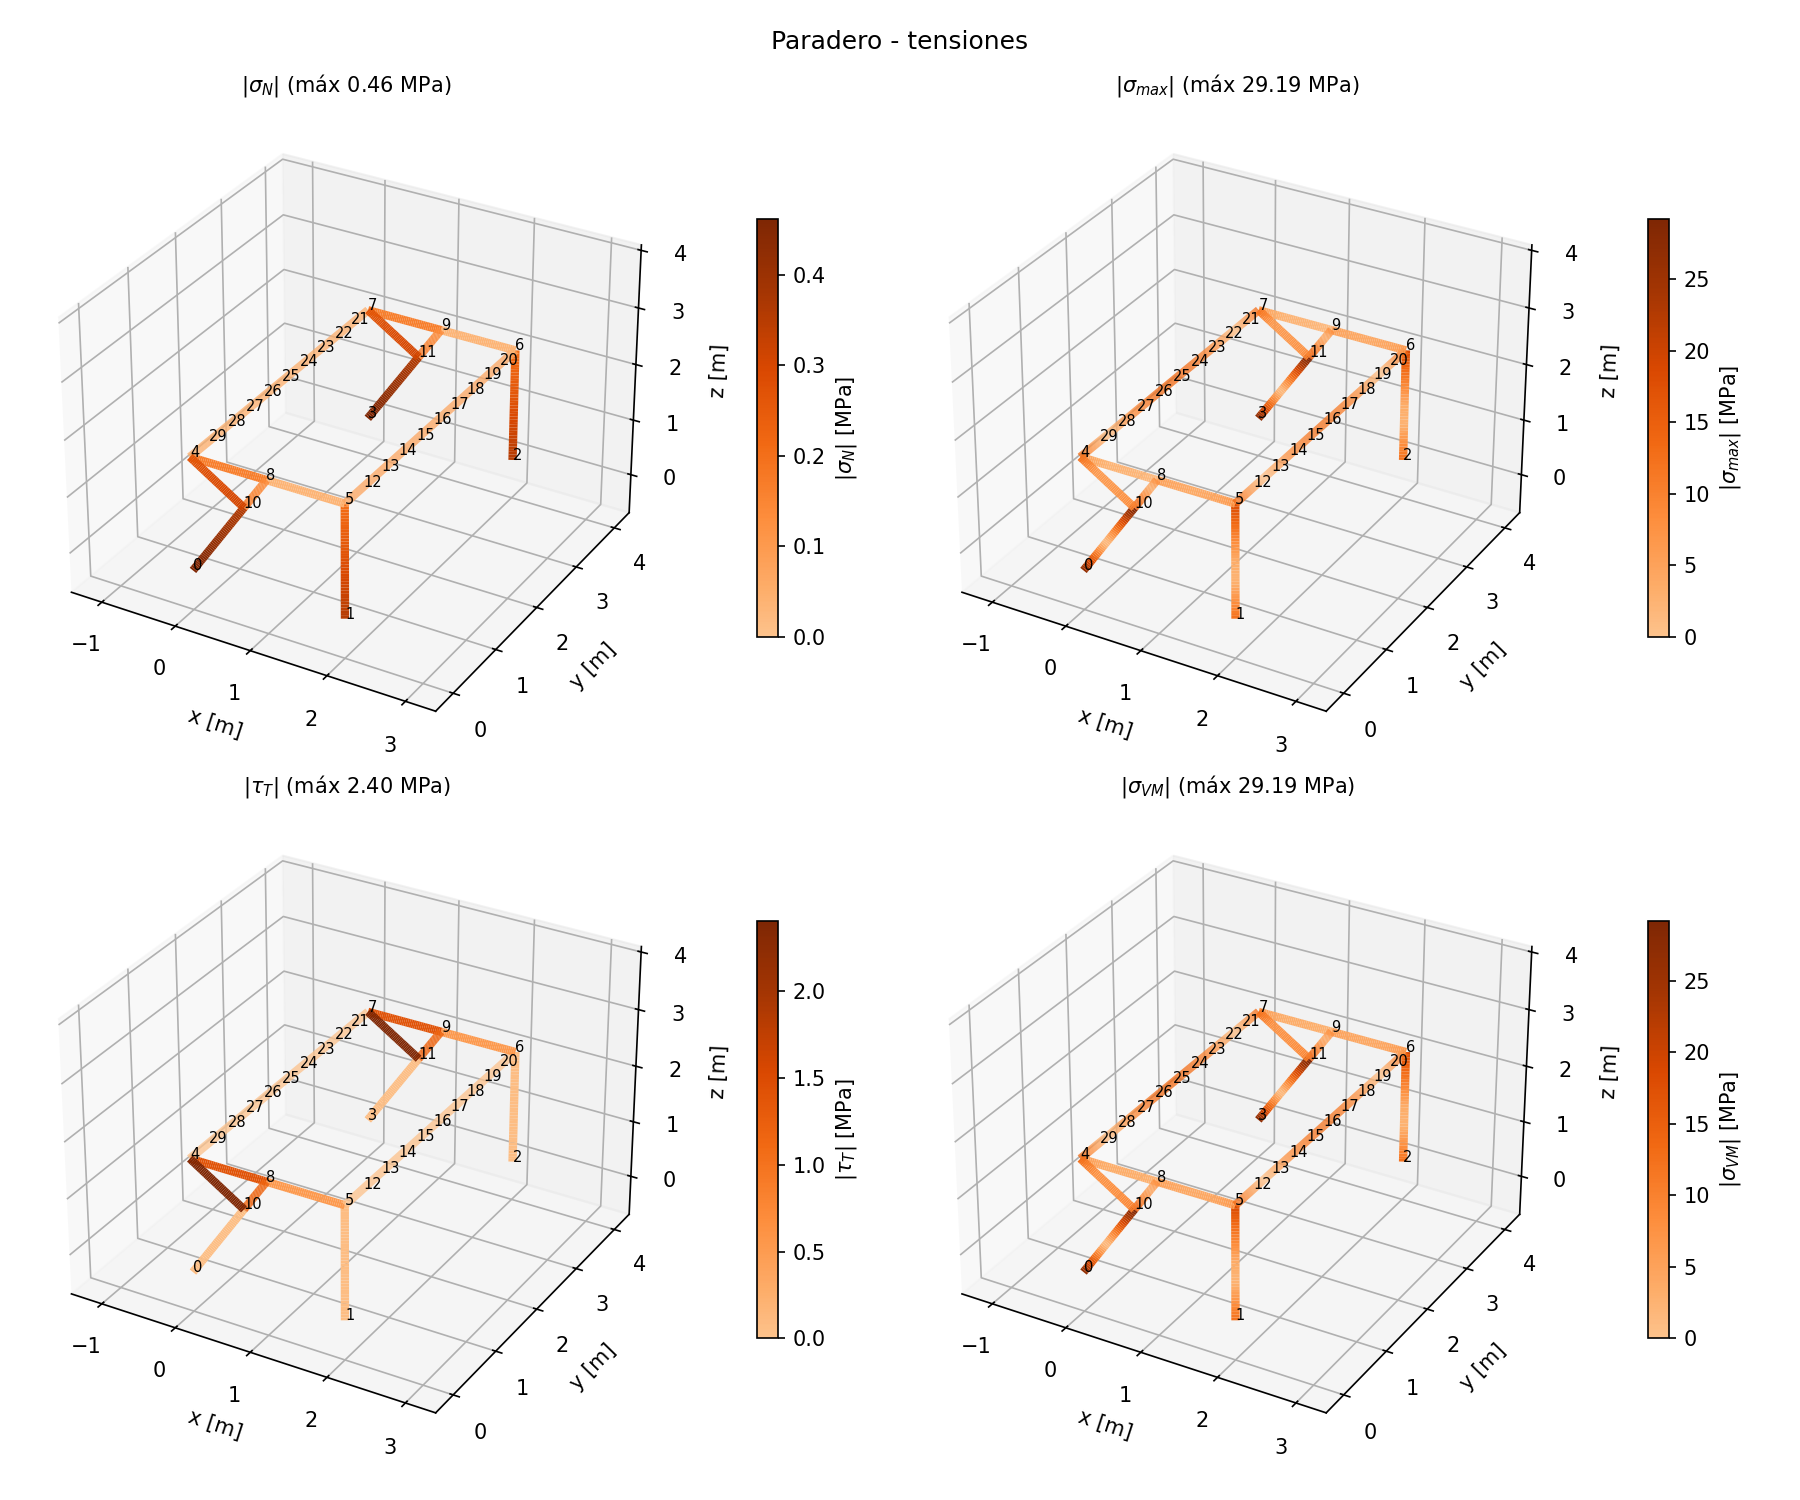
\includegraphics[width=\linewidth]{T2/figuras_P2/tensiones_3d.png}
\captionof{figure}{Tensiones sobre la estructura: normal por axial, normal
máxima, corte por torsión y von Mises. El color se asigna con el promedio
de cada segmento, por eso el máximo del gráfico (30.0 MPa) es algo menor que
el valor puntual en los nodos 10 y 11 (30.7 MPa).}
\label{fig:t2-p2-tensiones}
\end{center}

\begin{center}
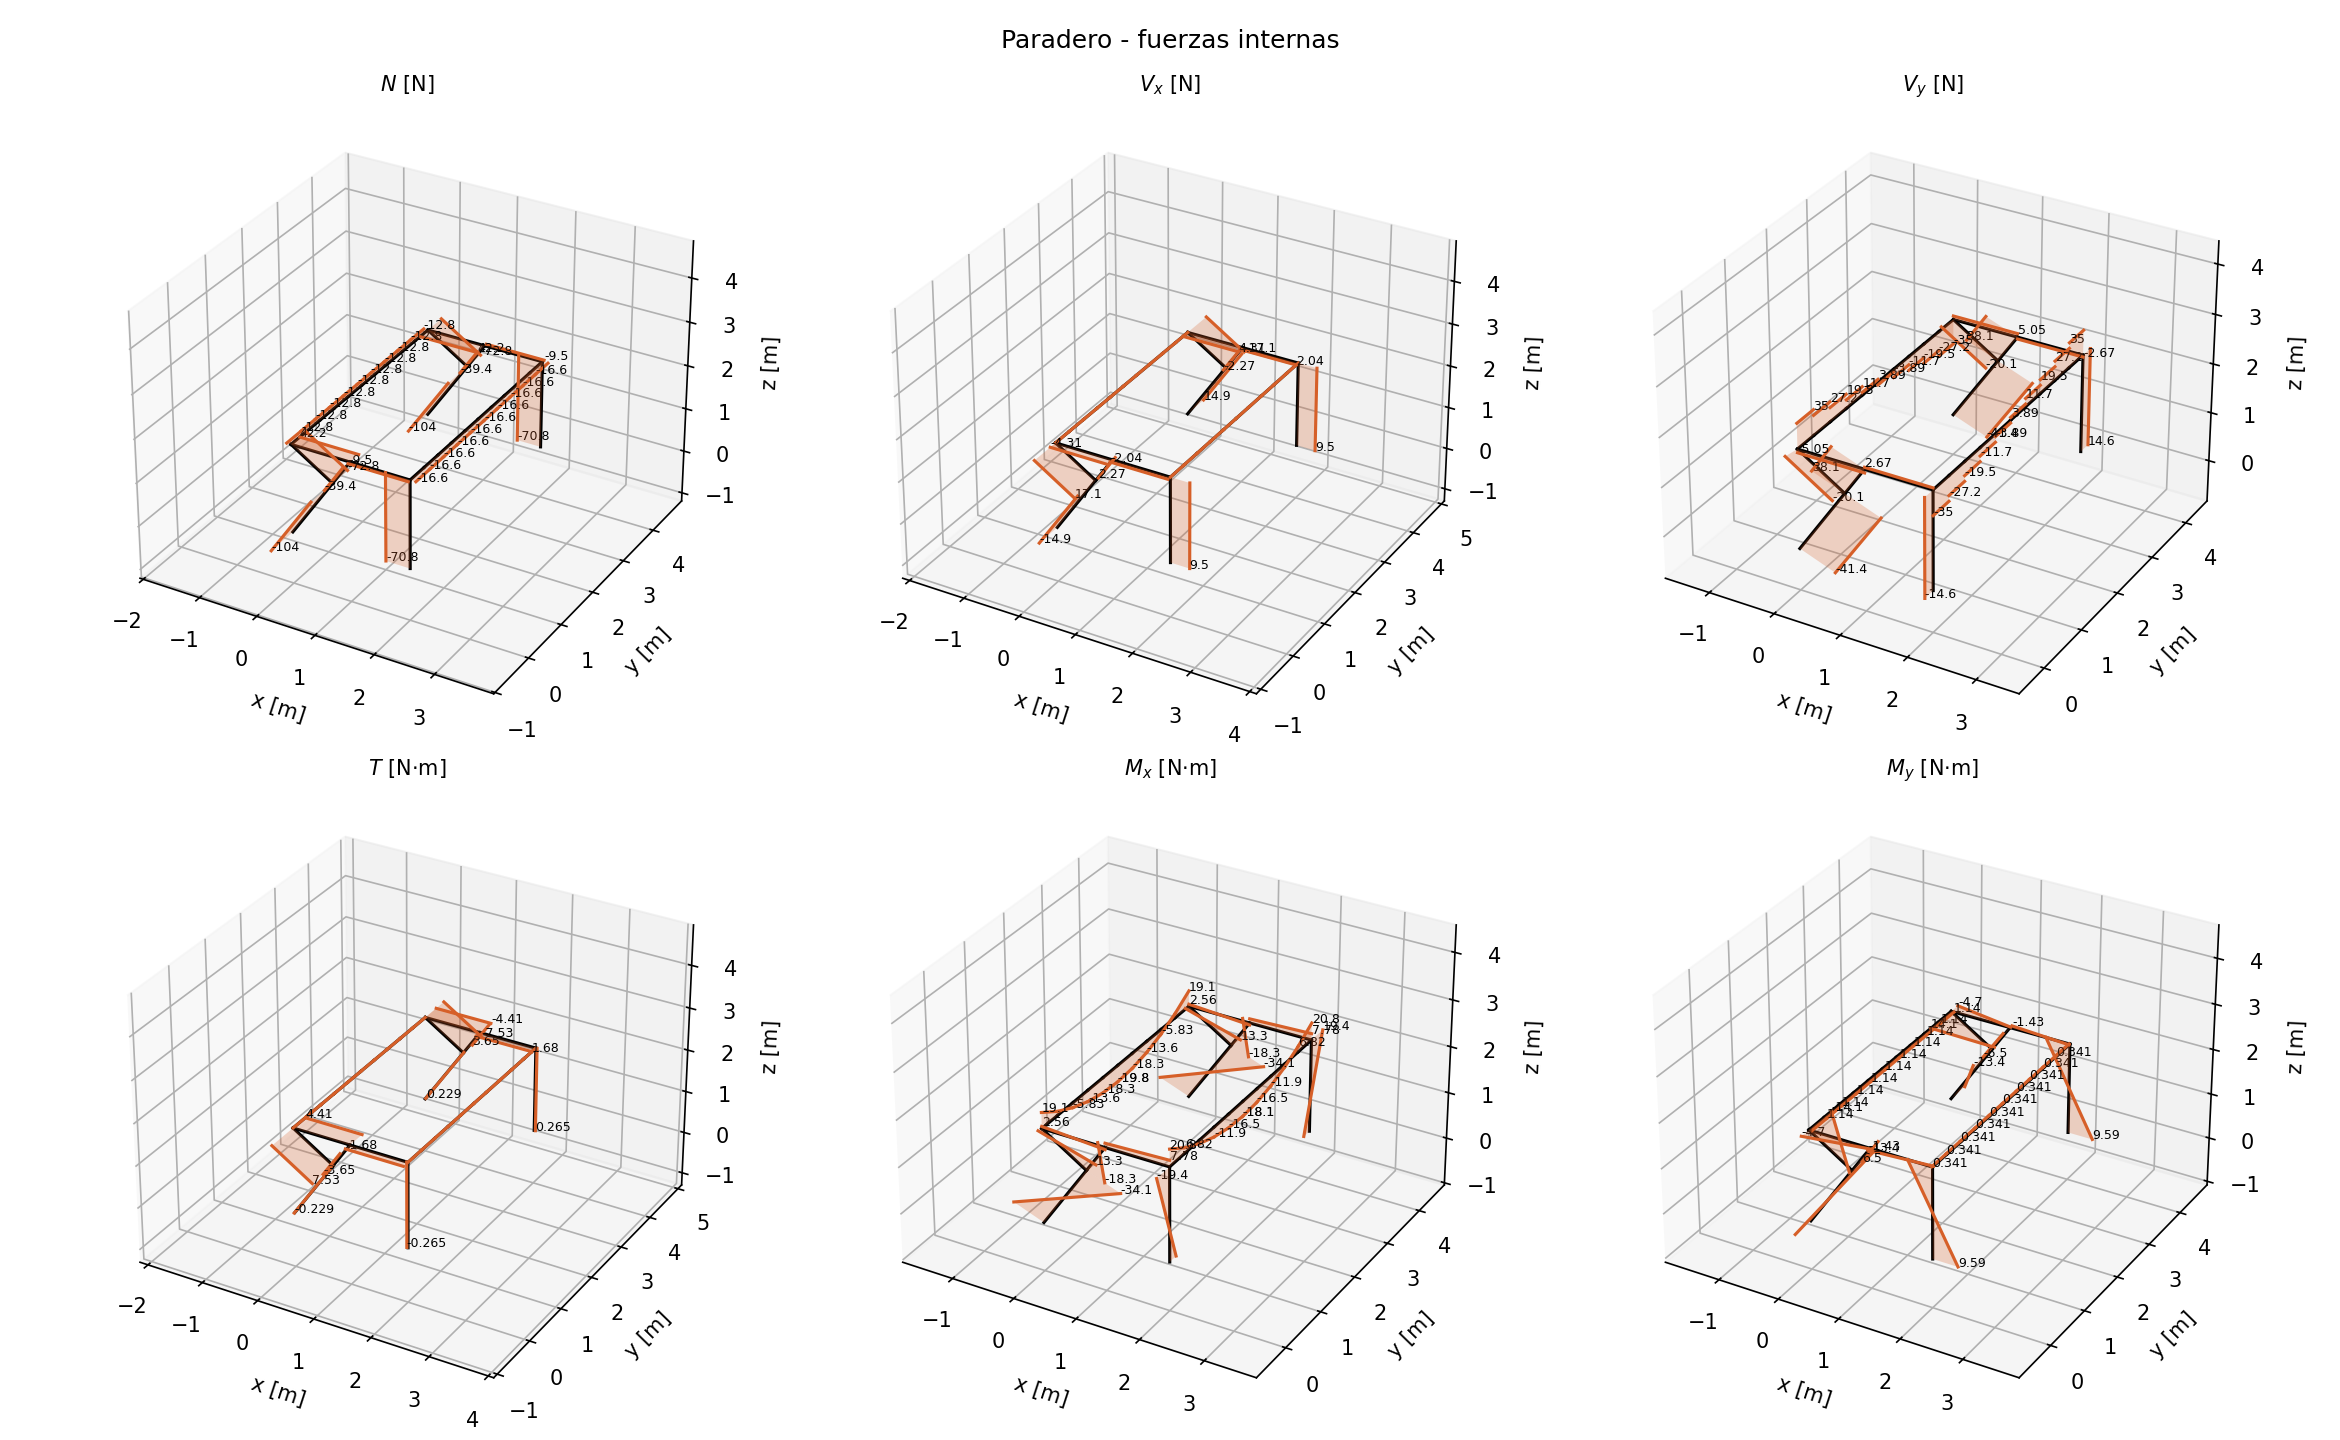
\includegraphics[width=\linewidth]{T2/figuras_P2/fuerzas_3d.png}
\captionof{figure}{Fuerzas internas en ejes locales sobre la estructura.}
\label{fig:t2-p2-fuerzas}
\end{center}

\begin{center}
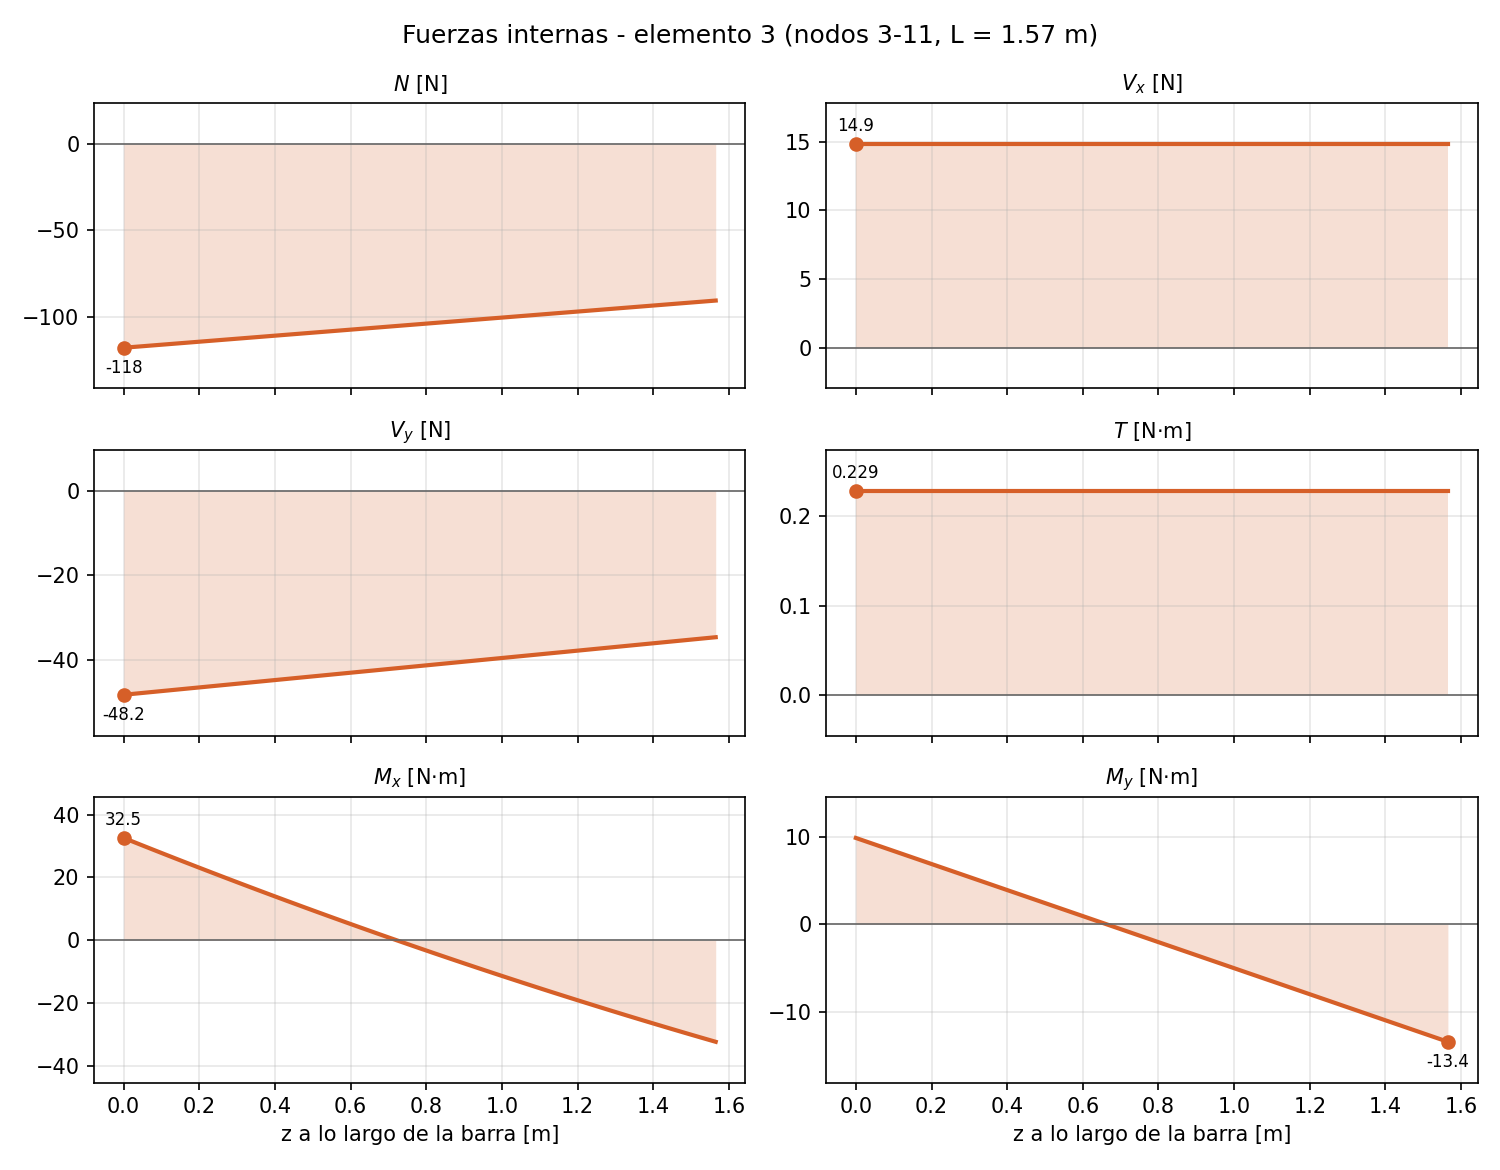
\includegraphics[width=0.85\linewidth]{T2/figuras_P2/barra_03_fuerzas.png}
\captionof{figure}{Fuerzas internas en la barra crítica (tramo inferior de
la columna inclinada, nodos 3--11). Como la carga está en los nodos, $N$ y
los cortes son constantes y los momentos lineales. El máximo de
$|M_x|+|M_y|$ está en el extremo superior ($z=L$).}
\label{fig:t2-p2-critica}
\end{center}

\begin{center}
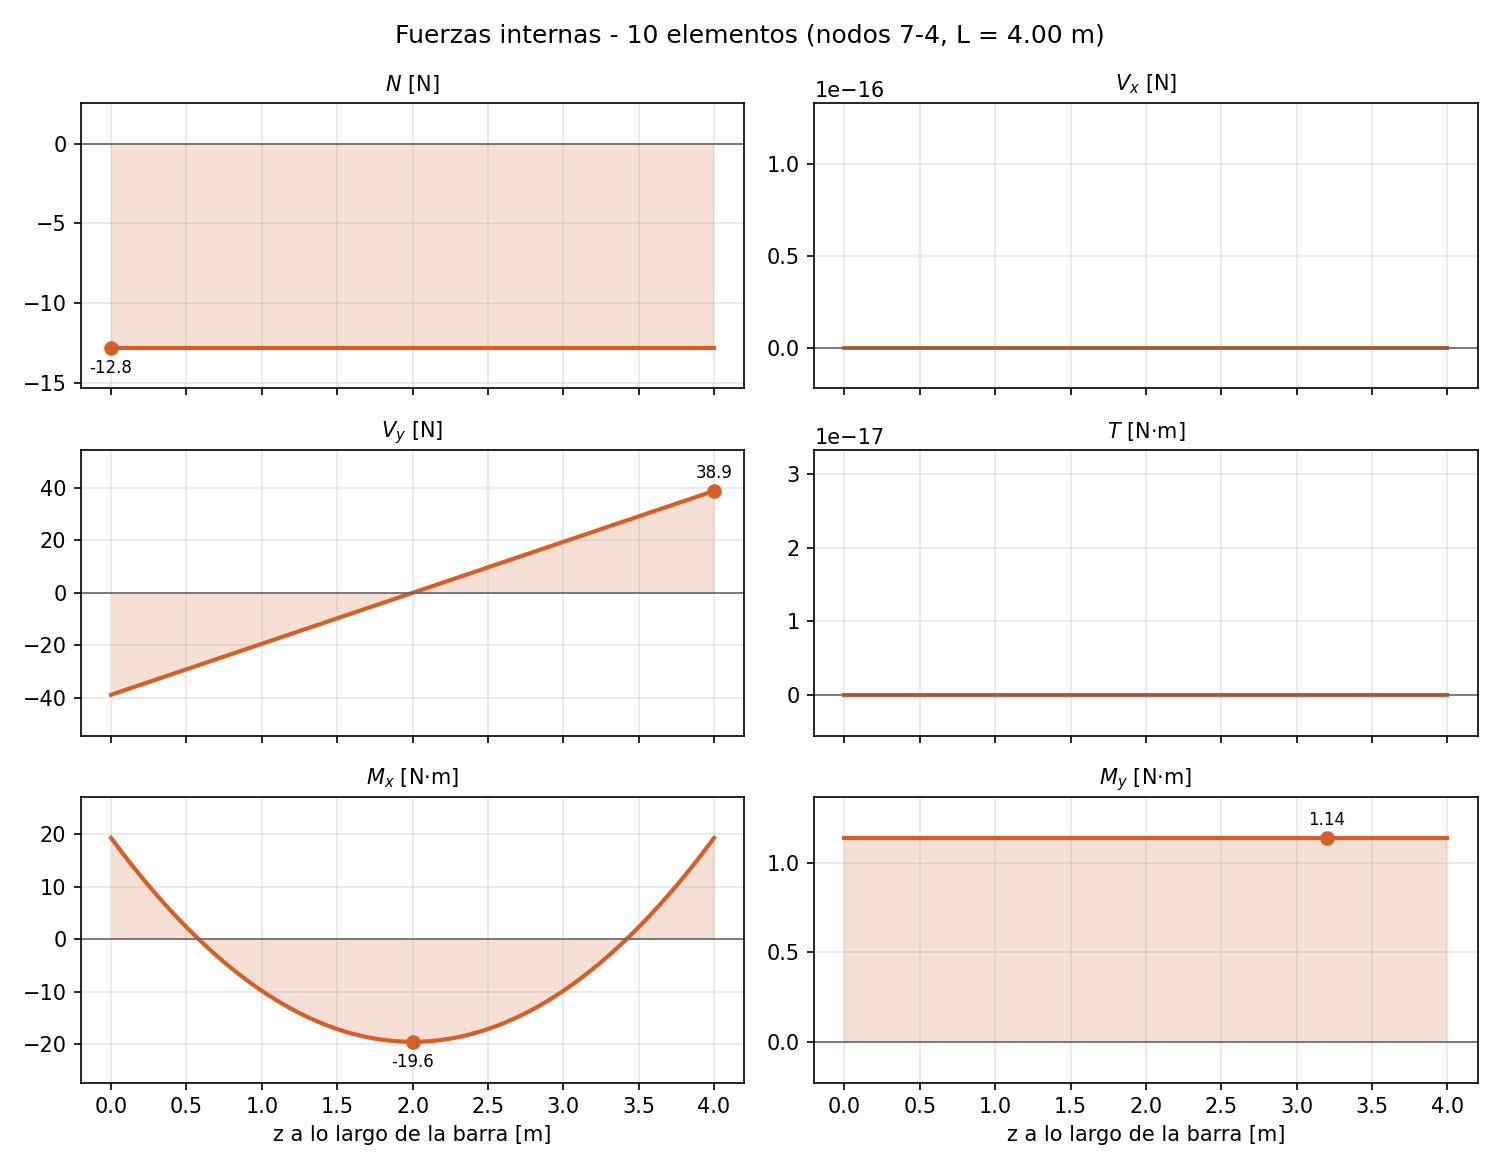
\includegraphics[width=0.85\linewidth]{T2/figuras_P2/barra_09_fuerzas.png}
\captionof{figure}{Fuerzas internas en el larguero trasero (nodos 7--4).
Con el peso aplicado en los 11 nodos, el corte baja en escalones de
$q\cdot0.4=7.78$ N en cada nodo y el momento es una poligonal que pasa
por sus valores nodales.}
\label{fig:t2-p2-larguero}
\end{center}
\end{desarrollo}

\begin{desarrollo}{Conclusión}
El diseño propuesto cubre $2\times4$ m a 2 m de altura con 22.3 m de tubo
Ø30$\times$3 (44 kg). Cumple ambas restricciones:
$\delta_{max}=7.36$ mm $<10$ mm y $\sigma_{VM,max}=30.7$ MPa $<300$ MPa
(FS $=9.8$). La restricción que controla es la deflexión y no la
resistencia, por lo que para este tubo el diseño se rige por rigidez. Los
atiesadores laterales de 0.92 m fueron la clave: redujeron la flecha
máxima en un 51\,\% (de 15.1 a 7.4 mm) agregando solo 1.8 m de tubo, y sin
tapar la vista frontal ni trasera del paradero.
\end{desarrollo}
